\documentclass[aspectratio=169]{beamer}
\usepackage{mathtools}
\usepackage{multirow}
\usepackage{multicol}
\newcommand{\pd}[2]{\frac{\partial #1}{\partial #2}}
\newcommand{\abs}[1]{\left|#1\right|}

\begin{document}
	\frame{
		\centering
		\Huge
		One- and Two-Dimensional Poisson's Equation
		\\\vspace{1.2cm}
		\large Pierce Hunter, Nick Kuckuck, Haoran Wang
		\\\vspace{0.8cm}
		\normalsize CIS 410/510 Final Presentation
		\\ 8$ ^{\text{th}} $ June 2020
	}
	\frame{
		\frametitle{Outline}
		\begin{enumerate}
			\item Theory
			\begin{itemize}
				\item Poisson in 1D
				\item Poisson in 2D
				\item Equations
				\item Discretizations
				\item Matrix formulations
			\end{itemize}
			\item Code samples
			\begin{itemize}
				\item $ A $ matrices and array set-up
				\item The four tests we run
				\item How we check for convergence
			\end{itemize}
			\item Results
			\begin{itemize}
				\item One dimensional with convergence test
				\item Two dimensional with error analysis
			\end{itemize}
		\end{enumerate}
	}
	\frame{
		\frametitle{One-dimensional model}
		We first solved Poisson's equation in 1D
		\begin{equation*}
			\pd{^2u}{z^2} = -1; \quad 0\leq z\leq 1
		\end{equation*}
		with boundary conditions
		\begin{equation*}
			\pd{u}{z}\left(1\right) = 0; \quad u(0) = 0
		\end{equation*}
		in the four following ways (all using built-in functions):
		\begin{itemize}
			\item Direct solve on the CPU
			\item CG on the CPU
			\item Direct solve on the GPU
			\item CG on the GPU
		\end{itemize}
	}
	\frame{
		\frametitle{1D Discretization}
		Use centered difference for $ z $
		\begin{equation*}
			\frac{u_{j-1}-2u_j+u_{j+1}}{\Delta z^2} = -1 ~~\text{for}~~ 1\leq j\leq N
		\end{equation*}
		Apply boundary conditions giving the system of equations
		\begin{equation*}
			\begin{dcases}
			\frac{-2u_2 + u_3}{\Delta z^2} = -1\\
			\frac{u_{j-1}-2u_j+u_{j+1}}{\Delta z^2} = -1;& 3\leq j\leq N-1\\
			\frac{u_{N-1} - u_N}{\Delta z^2} = -1
			\end{dcases}
		\end{equation*}
	}
	\frame{
		\frametitle{Matrix formulation}
		We can represent this system of equations as a matrix ($ A $) of the form
		\begin{equation*}
			A = \frac{1}{\Delta z^2}\begin{bmatrix}
			-2&1&0&\cdots&0\\
			1&-2&1&\cdots&0\\
			\vdots&\ddots&\ddots&\ddots&\vdots\\
			0&\cdots&1&-2&1\\
			0&\cdots&0&1&-1
			\end{bmatrix}
		\end{equation*}
		with the $ u $-column vector and $ b $-solution vector as
		\begin{equation*}
			u = \begin{bmatrix}
			u_2\\
			\vdots\\
			u_N
			\end{bmatrix} \qquad b = \begin{bmatrix}
			-1\\\vdots\\-1
			\end{bmatrix}
		\end{equation*}
		such that $ Au = b $
	}
	\frame{
		\frametitle{Two-dimensional approach}
		In 2D Poisson's equation is
		\begin{equation*}
			\pd{^2u}{y^2} + \pd{^2u}{z^2} = -1; \quad \begin{dcases}
			0\leq y\leq 1\\
			0\leq z\leq 1
			\end{dcases}
		\end{equation*}
		and we now apply boundary conditions on edges as
		\begin{align*}
			\pd{u}{y} = 0&\text{ at }y=1\\
			\pd{u}{z} = 0&\text{ at }z=1\\
			u = 0&\text{ at }y=0\vphantom{\pd{u}{y}}\\
			u = 0&\text{ at }z=0\vphantom{\pd{u}{y}}
		\end{align*}
	}
	\frame{
		\frametitle{2D Discretization}
		Using centered-difference for $ y $ and $ z $
		\begin{equation*}
			\frac{u_{i-1,j} - 2u_{i,j} + u_{i+1,j}}{{\Delta y}^2} + \frac{u_{i,j-1} - 2u_{i,j} + u_{i,j+1}}{{\Delta z}^2} = -1
		\end{equation*}
		which simplifies when $ \Delta y = \Delta z $ to
		\begin{equation*}
			u_{i-1,j} + u_{i,j-1} - 4u_{i,j} + u_{i+1,j} + u_{i,j+1} = -{\Delta y}^2
		\end{equation*}
		\begin{equation*}
			2\leq i\leq N;\qquad 2\leq j\leq N
		\end{equation*}
	}
	\frame{
		\frametitle{2D Matrix formulation}
		Define a global index $ k $ as
		\begin{equation*}
			k = (i-2)(N-1) + (j-1)
		\end{equation*}
		Then create
		\begin{itemize}
			\item $ (N-1)^2\times(N-1)^2 $ matrix $ A $
			\item $ (N-1)^2\times1 $ array $ b $
		\end{itemize}
		Solve for
		\begin{itemize}
			\item $ (N-1)^2\times1 $ solution vector $ u $
		\end{itemize}
	}
	\frame{
		\frametitle{2D Matrix $ A $}
		The matrix $ A $ contains
		\begin{itemize}
			\item -4 along the main diagonal, except
			\begin{itemize}
				\item -3 for row $ \alpha(N-1) $, $ 1\leq \alpha\leq N-2 $
				\item -3 for row $ \left(N-2\right)\left(N-1\right)+\beta $, $ 1\leq\beta\leq N-2 $
				\item -2 for row $ \left(N-1\right)^2 $
			\end{itemize}
			\item 1 along four subdiagonals
			\begin{itemize}
				\item $ j-1 $ except $ (\alpha(N-1)+1,\alpha(N-1)) $, $ 1\leq\alpha\leq N-2 $
				\item $ j+1 $ except $ (\alpha(N-1),\alpha(N-1)+1) $, $ 1\leq\alpha\leq N-2 $
				\item $ i-1 $ (i.e. starting at $ (N,1) $)
				\item $ i+1 $ (i.e. starting at $ (1,N) $)
			\end{itemize}
		\end{itemize}
	}
	\frame{
		\frametitle{Code Samples}
	
	}
	\frame{
		\frametitle{1D Solution Vector}
		Our model solves for velocity $ u(z) $\\
		\begin{minipage}{.6\textwidth}
			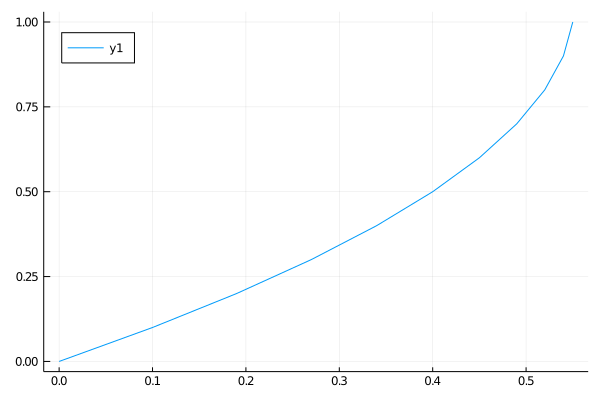
\includegraphics[width=\linewidth]{1D_mid_res.png}
		\end{minipage}
		\begin{minipage}{.39\linewidth}
			\begin{itemize}
				\item Velocity decreases with depth
				\item The boundary conditions are satisfied
				\begin{itemize}
					\item $ u(0)=0 $
					\item $ u'(1) = 0 $
				\end{itemize}
			\end{itemize}
		\end{minipage}
	}
	
	\frame{
		\frametitle{1D Convergence Test}
		\begin{center}
			\renewcommand{\arraystretch}{2.0}
			\begin{tabular}{c|c|c|c}
				\hline\hline
				$\displaystyle \Delta z $&$\displaystyle \varepsilon_{\Delta z} = \sqrt{z}\lVert u-e\rVert $&$ \displaystyle \Delta\varepsilon = \frac{\varepsilon_{2\Delta z}}{\varepsilon_{\Delta z}} $&$\displaystyle r = \log_2\left(\Delta\varepsilon\right) $\\
				\hline
				0.1&$3.102\times 10^{-2}$&N/A&N/A\\
				0.05&$1.497\times 10^{-2}$&2.072&1.051\\
				0.025&$7.352\times 10^{-3}$&2.036&1.026\\
				0.0125&$3.642\times 10^{-3}$&2.019&1.014\\
				\hline
			\end{tabular}
		\end{center}
	}
	\frame{
		\frametitle{1D Time Analysis}
		Using $ \Delta z = 5\times10^{-5} $
		\begin{center}
			\renewcommand{\arraystretch}{1.5}
			\begin{tabular}{c|c|c|c}
				\hline\hline
				\textbf{Device}&\textbf{Method}&\textbf{Time [s]}&\textbf{Error~~$\sqrt{z}\lVert u-e\rVert $}\\
				\hline
				\multirow{2}{*}{CPU}&Direct&0.0426&$1.44\times 10^{-5}$\\
				&CG&15.1&$1.44\times 10^{-5}$\\
				\hline
				\multirow{2}{*}{GPU}&Direct&1.13&$1.44\times 10^{-5}$\\
				&CG&3.19&$1.44\times 10^{-5}$\\
				\hline
			\end{tabular}
		\end{center}
		Direct CPU solve is by far the fastest method at this problem size
	}
	\frame{
		\frametitle{2D Results}
		No analytical solution, so we test for convergence
		\begin{enumerate}
			\item Visually
			\item Via $ Au-b \approx 0 $
		\end{enumerate}
	}
	\frame{
		\frametitle{2D Visual Comparison}
		\begin{center}
			\begin{minipage}{.7\linewidth}
				Low resolution ($ \Delta z = 0.1 $)\\
				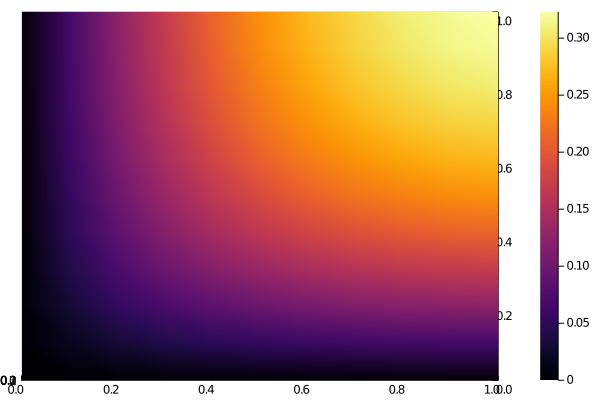
\includegraphics[width=\linewidth]{2D_low_res}
			\end{minipage}
		\end{center}
	}
	\frame{
		\frametitle{2D Visual Comparison}
		\begin{center}
			\begin{minipage}{.7\linewidth}
				Mid resolution ($ \Delta z = 0.025 $)\\
				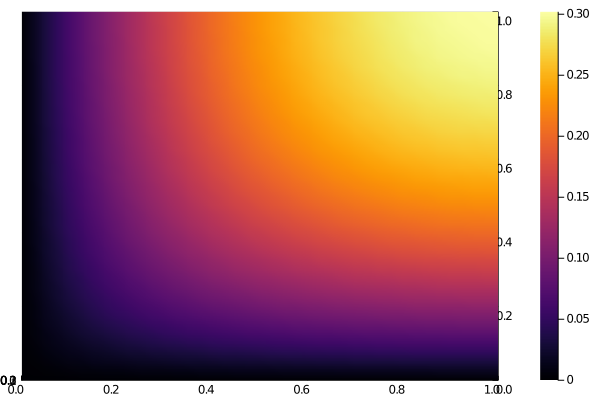
\includegraphics[width=\linewidth]{2D_mid_res}
			\end{minipage}
		\end{center}
	}
	\frame{
		\frametitle{2D Visual Comparison}
		\begin{center}
			\begin{minipage}{.7\linewidth}
				\small High resolution ($ \Delta z = 0.01 $)\\
				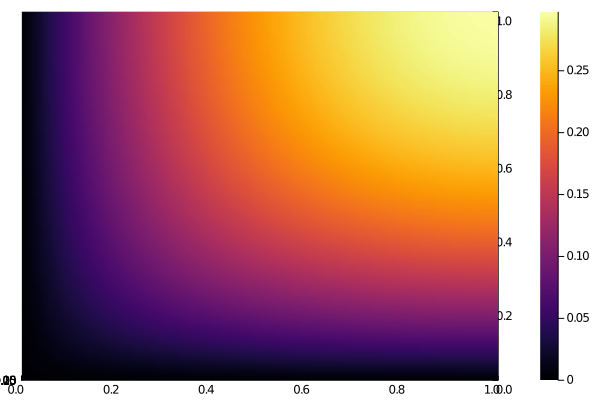
\includegraphics[width=\linewidth]{2D_high_res}
			\end{minipage}
		\end{center}
	}
	\frame{
		\frametitle{2D Error Analysis}
		Solve for $ u $, and check $ Au - b \approx 0 $
		\begin{center}
			\renewcommand{\arraystretch}{2.0}
			\begin{tabular}{c|c}
				\hline\hline
				$\displaystyle \Delta z $&$\displaystyle Au-b $\\
				\hline
				0.1&$8.02\times 10^{-16}$\\
				0.05&$1.8\times 10^{-15}$\\
				0.025&$4.6\times 10^{-15}$\\
				0.0125&$1.02\times 10^{-14}$\\
				\hline
			\end{tabular}
		\end{center}
		The error seems to be something on the order of $ (N-1)^2\varepsilon $ with $ N $ as $ 1/\Delta z $ and $ \varepsilon $ machine precision.
	}
	\frame{
		\frametitle{2D Time Analysis}
		\begin{center}
			\renewcommand{\arraystretch}{1.5}
			\begin{tabular}{c|c|c|c}
				\hline\hline
				\textbf{Device}&\textbf{Method}&\textbf{Time [s]}&\textbf{Error~~$Au-b $}\\
				\hline
				\multirow{2}{*}{CPU}&Direct&0.027&$1.31\times 10^{-14}$\\
				&CG&0.025&$1.49\times 10^{-10}$\\
				\hline
				GPU&CG&0.2&$1.49\times 10^{-10}$\\
				\hline
			\end{tabular}
		\end{center}
		\begin{itemize}
			\item CG is less precise
			\item The CPU methods are faster
			\item Likely due to problem size limitations
			\item GPU should surpass CPU eventually, but limited by GPU memory on Talapas
		\end{itemize}
	}
\end{document}